%*******************************************************************************
%****************************** Second Chapter *********************************
%*******************************************************************************

\chapter{Theoretical Model and Numerical Simulation Methods}
\graphicspath{{Chapter2/Figs/}}

To model the chromosome movements during nuclear osculation in fission yeast, let us start from a single chromosome modeled by a single polymer loop. 
In this chapter, we will introduce the details of the polymer model for the chromosomes and the simulation methods that resolving the dynamics and statistics of the polymer. 


%********************************** %First Section  **************************************
\section{Stochastic models of polymer loops}
\label{sec:stochastic_models_of_polymer_loops}

As mentioned in the previous chapter, there are three pairs of chromosomes in fission yeast. During nuclear oscillation, these three pairs of chromosomes bound to one point, i.e. the Spindle Pole Body (SPB). Now let us start with the simplest case and neglect the interactions between chromosomes, think about a single chromosome. It is a polymer with the ring structure, and an external force is exerted on the SPB. We have two choices to model this chromosome, i.e. the bead-rod model or the bead-spring model. We will use both models in this thesis but more discussions are focused on the bead-rod. Both models have their own benefits and shortcomings. Computationally, it is easier to manipulate the bead-spring model than the bead-rod. However, the bead-rod has the intrinsic property of finite extensible without resorting to some complex nonlinear spring potentials. This benefit we think is important because the chromosomes are highly condensed and are definitely finite extensible. In fact, we will show that the finite extensibility takes an important role for the polymer dynamics, see in the later chapters. And the simplicity of bead-rod model offers us the possibility to find analytical solutions. 

In this section, we will introduce both the bead-rod and bead-spring model for modeling the chromosomes. However, before that, let us first do a coordinate transformation that makes our analysis much easier. 

\subsection{Coordinate transformation}
\label{sub:coordinate_transformation}
Let us consider a single chromosome pulled at the SPB. The pulling force drives the chromosome moves with a velocity $\mathbf{v}$. In our model, the SPB is modeled as one monomer in the polymer loop. Other monomers representing the chromosome move together with the SPB because of the bonds. This scenario of pulled polymer loop is shown in Fig. \ref{fig:coordinate} (a). 
\begin{figure}[htpb]
    \centering
    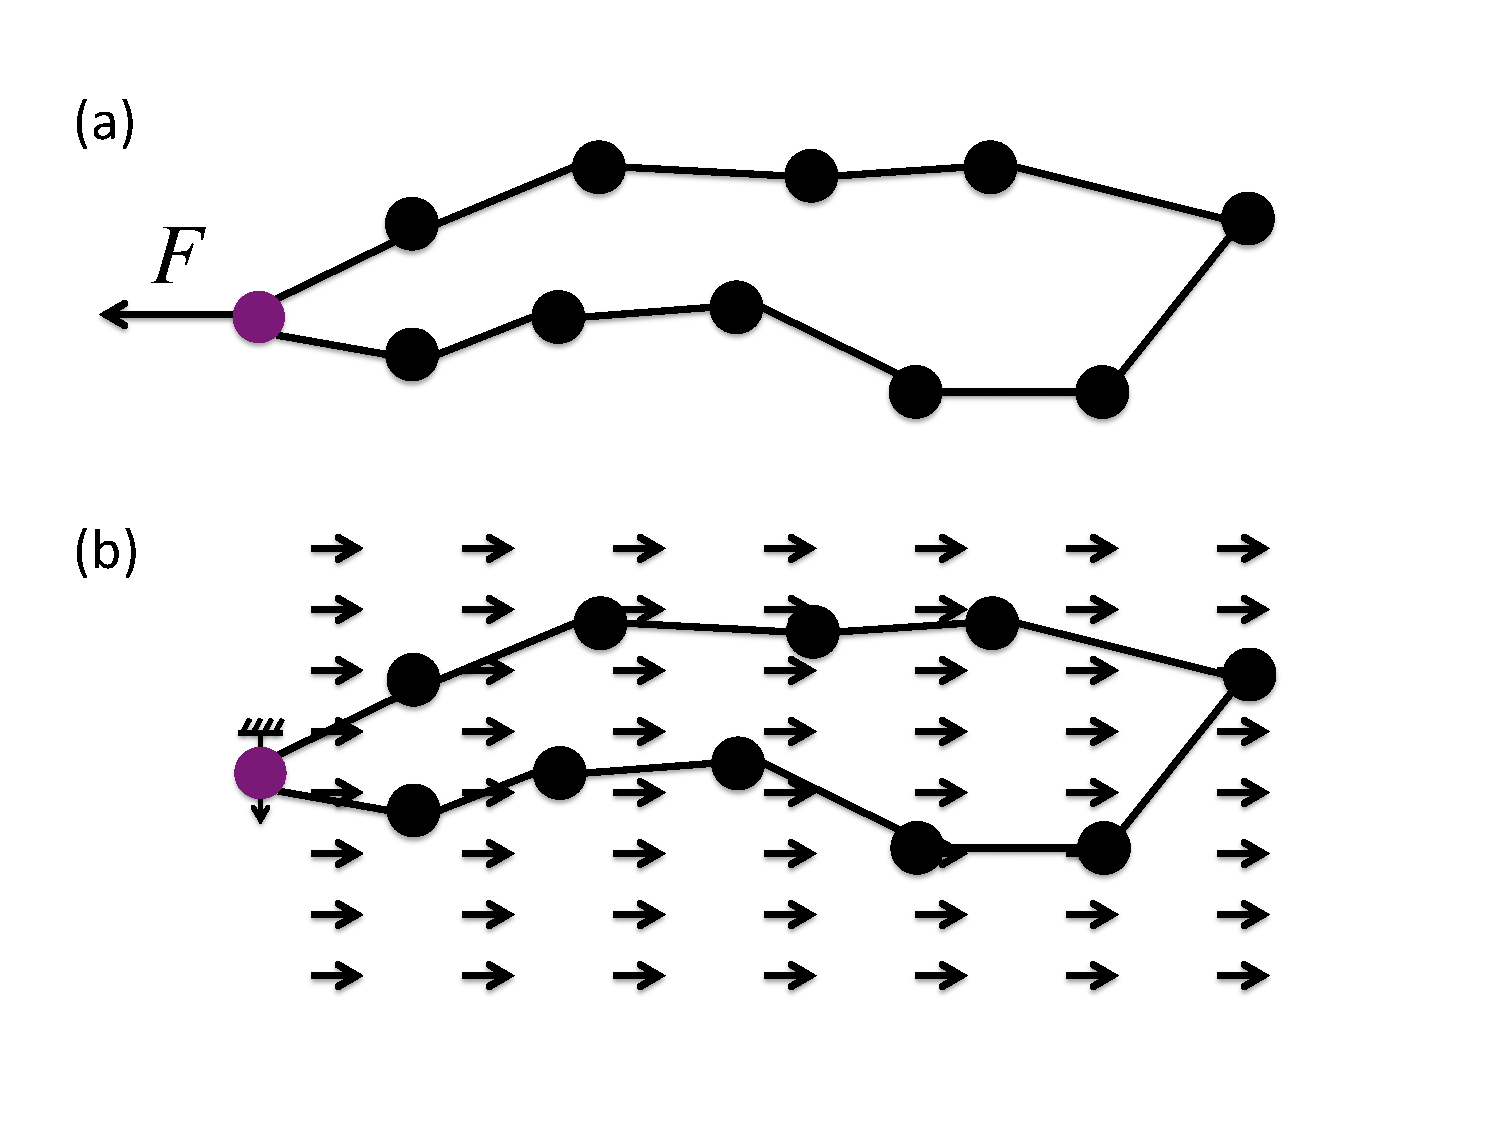
\includegraphics[width=0.8\linewidth]{coordinate}
    \caption{Illustration of coordinate transformation. (a) a pulled polymer loop before transformation; (b) pinned polymer loop in an external field after transformation. }
    \label{fig:coordinate}
\end{figure}

Now let us imagine we are sitting on the SPB. Then effectively, the SPB is pinned, and the polymer loop is immersed in a flow with velocity $-\mathbf{v}$, see in Fig. \ref{fig:coordinate} (b). Let us assume the Stoke's law is valid and according to that, there is a force $\mathbf{F}^e = - \xi \mathbf{v}$ exerting on every bead. $\xi$ is the friction coefficient for the bead in the solution.

In conclusion, the pulled polymer loop model is equivalent to the pinned polymer loop in an external force field. In our analysis, we will use the pinned polymer loop picture, because it is more easily to deal with both numerically and analytically. In the simulation, an extreme large pulling force is required if we use the first picture. The unusual force can easily become the bottleneck for the choosing of the integration time step. In theory, the force field picture offers a very clean energy landscape. Thus the pinned picture is preferred in out study. 

\subsection{Bead-rod model}
\label{sub:bead_rod_model}
Now let us come to a concrete polymer model for modeling the chromosomes, i.e. the bead-rod model. For this model, the beads representing chromosome segments are connected by the massless rigid rod. For simplicity, we assume the length of every rod is identical, denote by $a$. The rigidity of the rod means the distance between two neighboring beads is fixed. 
\begin{figure}[htpb]
    \centering
    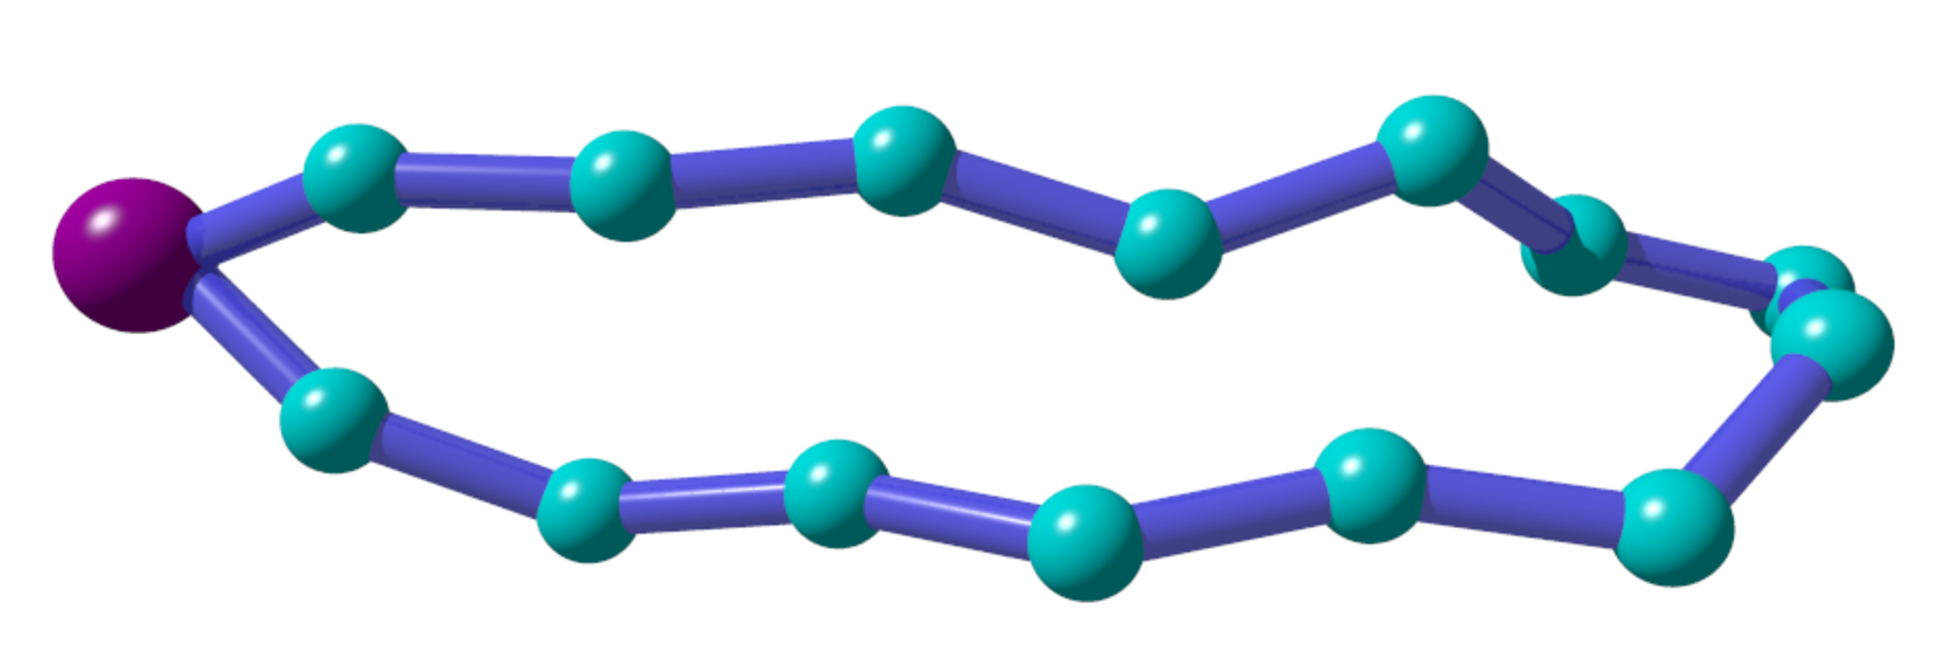
\includegraphics[width=0.8\linewidth]{beadrod}
    \caption{Sketch of the bead-rod loop model. The magenta bead represents the SPB and other cyan beads represent the chromosome segments.}
    \label{fig:beadrod}
\end{figure}

The dynamics of the polymer is specified by the motion of the beads. We shall first give out the dynamical equation and then explain how does it come from. Let us say the contour length of the polymer loop is $L$, i.e. there are $L$ beads (including the SPB) and $L$ rods in the polymer. Denote the beads by the index $i = 0, 1, 2,\cdots, L-1, L$. Notice that the periodic index is used due to the looping structure, i.e. for any indexing quantities $x_0 = x_L$. Then the dynamical equation of $i^{\rm {th}}$ bead can be written as
\begin{equation}
    \label{eq:beadrodEq}
    \xi \frac{d \mathbf{r}_i}{d t} = \mathbf{F}_i^{u} + \mathbf{F}_i^{c} + \mathbf{F}_i^{pseudo} + \mathbf{F}_i^{e} + \mathbf{F}_i^{b}
\end{equation}
where $\xi$ is the friction coefficient of the bead in the solution, $\mathbf{F}_i^{u}$ is the interaction force specified by some kind of potentials, $\mathbf{F}_i^{c}$ is the constraint force that keeps the rod length fixed, $\mathbf{F}_i^{e}$ is the external force and $\mathbf{F}_i^{b}$ is the Brownian force caused by thermal fluctuations. And what is left in the right hand of Eq. \eqref{eq:beadrodEq} is $\mathbf{F}_i^{pseudo}$, which is a special type of force introduced in the bead-rod model in order to get the correct statistics. We will discuss more about it later. 

Now let us come back to explain how does Eq. \eqref{eq:beadrodEq} come from.  Firstly, notice that $\mathbf{F}_i^b$ in the equation is a stochastic variable, so Eq. \eqref{eq:beadrodEq} is actually a stochastic differential equation. Secondly, the left-hand side of Eq. \eqref{eq:beadrodEq} is actually rearranged from the friction force of the bead in the solution $-\xi\mathbf{v}_i$. And we have assumed the solution is homogeneous so that the friction coefficient is independent of the space and time. Third, the inertial of the bead is neglected due to millions of collisions per second from the water molecules. In another word, Eq. \eqref{eq:beadrodEq} essentially can be written as $\mathbf{F}_i^{total} = \mathbf{0}$. This is simply the Newton's law with inertial neglected. This kind of dynamics is commonly used in polymer physics and called Brownian Dynamics \cite{Somasi2002,Cruz2012}. 

Let us now discuss each term of the right-hand side of Eq. \eqref{eq:beadrodEq} one by one. 

$\bullet$ Brownian force $\mathbf{F}_i^{b}$

The Brownian force can be caused by the enormous instantaneous collisions of the solvent molecules or by other sort of interactions between chromosomes and proteins in the nucleus. The level of fluctuation can be characterized by an effective temperature $T$. Mathematically, the Brownian force is described by a Gaussian process with the zero mean in space and time and the non-zero second moment, which can be written as:
\begin{subequations}
    \label{eq:brownianforce}
    \begin{equation}
        \left<\mathbf{F}_i^b\right> =\mathbf{0},
    \end{equation}
    \begin{equation}
        \left<\mathbf{F}_i^b(t)\mathbf{F}_j^b(t^{\prime})\right> = 2k_B T \xi \delta_{ij} \delta(t-t^{\prime}),
    \end{equation}
\end{subequations}
here, $\xi$ is the friction coefficient. $k_B$ is the Boltzmann constant. $\delta_{ij}$ is the Kronecker delta means there is no correlation for the Brownian force exerting on different beads. The second $\delta$ is the Dirac delta function. 

$\bullet$ External force $\mathbf{F}_i^{e}$

The external force in our pinned polymer loop model is simply the equivalent flow field after coordinate transformation. So we have $\mathbf{F}_i^e = \xi \mathbf{v}_{\rm{SPB}}$. In general, $\mathbf{v}_{\rm{SPB}} = \mathbf{v}_{\rm{SPB}}(t)$ is a function of time. However, when we consider the simplest case that the chromosome is pulled to move steadily in one direction, $\mathbf{v}_{\rm{SPB}}$ is a constant.

$\bullet$ Constraint force $\mathbf{F}_i^{c}$

The constraint force is the tension force on the rod to keep the length fixed. So the direction of the force is along the rod orientation. The rigid rod constraint can be written as 
\begin{equation}
    \label{eq:rodConstraint}
    |\mathbf{r}_{i} - \mathbf{r}_{i-1}| - a = 0,
\end{equation}
and $\mathbf{r}_{0} = \mathbf{r}_L$ for the periodic indexing. The constraint force is an implicit force that depends on the other force exerting on the beads. We will discuss how to calculate this force in next section. 

$\bullet$ \emph{Pseudo} force $\mathbf{F}_i^{pseudo}$

The \emph{Pseudo} force is a special virtual force that added in order to obtain the statistics we want. If we neglect the bending energy, excluded volume effect and other complex interactions in the model, we are essentially talking about the simplest freely joint polymer model. For such a simple model, we expect the random walk statistics, i.e. the orientation of two consecutive rods is independent. So the distribution of the included angle of two rods should be uniform. However, we cannot obtain this statistics as we want without the \emph{pseudo} force.

Let us take a simple example, the distribution of included angle of a trimer in 3D. Denote the angle as $\theta$. The 3D spherical uniform distribution can be written as
\begin{equation}
    \label{eq:trimerUniform}
    p(\theta) = const. \sin\theta.
\end{equation}
On the other hand, the distribution of rigid bead-rod trimer without \emph{pseudo} force can be derived using the generalized coordinate
\begin{equation}
    \label{eq:trimerRigid}
    p(\theta) = const. (1-\frac{1}{4}\cos^2\theta)^{1/2}\sin\theta.
\end{equation}
So they are not the same as we see here. The reason for this discrepancy is the rigidity of constraints reduce the phase space of the trimer from $6$ dimensional gully to $4$ dimension manifold. The simple Brownian force ensures the probability is uniform among the manifold but not $\theta$. 
\begin{figure}[htpb]
    \centering
    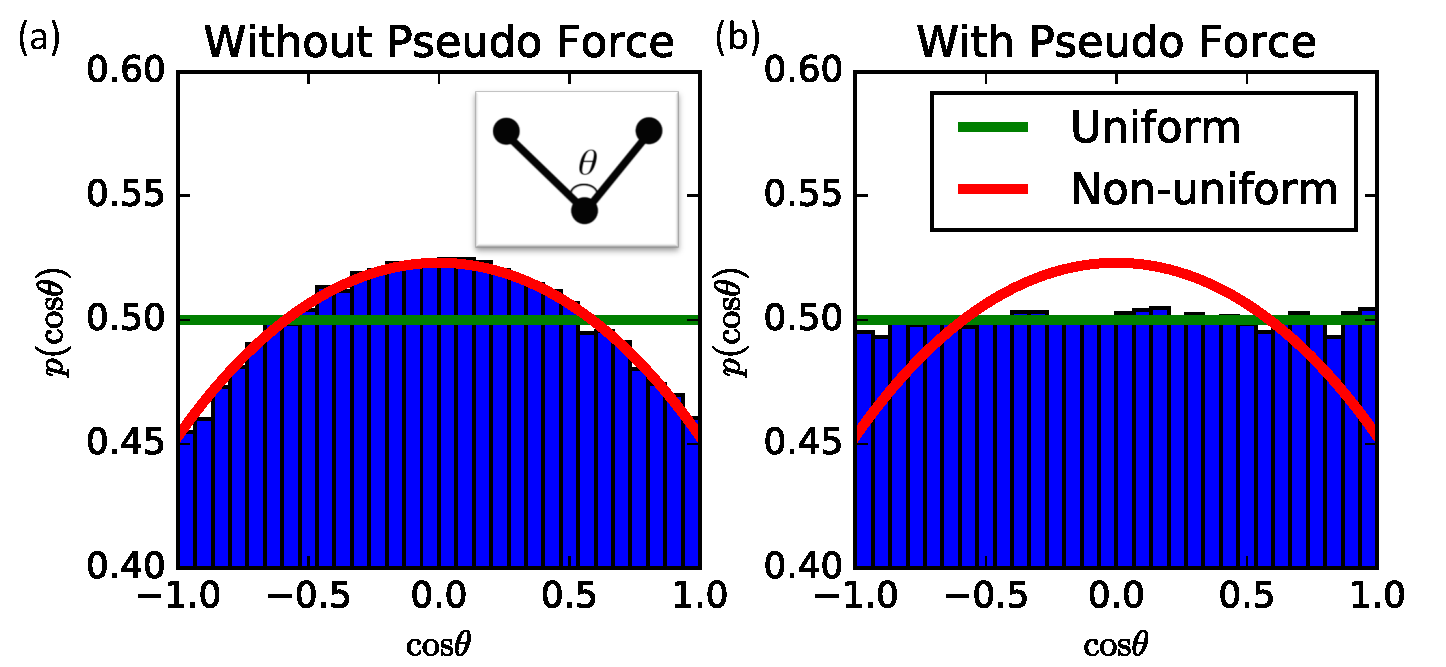
\includegraphics[width=1.0\linewidth]{trimer}
    \caption{The distribution of included angle of a bead-rod trimer. (a) without \emph{pseudo} force; (b) with \emph{pseudo} force. The blue bins are from Brownian Dynamics simulation results. Inset of (a) is a sketch for the trimer. }
    \label{fig:trimer}
\end{figure}

To solve the problem and obtain the statistics we want, Fixman introduced an effective \emph{pseudo} potential depends on the polymer configuration \cite{Fixman1974}, and hence we have a \emph{pseudo} force in Eq. \eqref{eq:beadrodEq}. The explicit form of the \emph{pseudo} force can be written as
\begin{subequations}
    \label{eq:pseudoForce}
    \begin{equation}
        \mathbf{F}_i^{pseudo} = -\frac{\partial U_{met}}{\partial\mathbf{r}_i},
    \end{equation}
    \begin{equation}
        U_{met} = \frac{1}{2}k_B T \ln(\det \mathbf{G}),
    \end{equation}
\end{subequations}
where $\mathbf{G}$ is the metric matrix of the bead-rod system \cite{Pasquali2002}. We will show the details for the calculation of \emph{pseudo} force in next section.

$\bullet$ Other potential forces $\mathbf{F}_i^{u}$

Other potential forces count the forces derived from bending energy, excluded volume effect, hydrodynamical interaction and other interaction potentials. The general form of this force can be written as
\begin{equation}
    \label{eq:potentialForce}
    \mathbf{F}_i^{u} = -\sum_{U}\frac{\partial U}{\partial\mathbf{r}_i},
\end{equation}
here $U$ can be different potentials. For instance, the bending potential can be calculated as 
\begin{equation}
    \label{eq:bending}
    U_{bend} = - \frac{\kappa}{a} \sum_{i=1}^{L} \mathbf{u}_i \cdot \mathbf{u}_{i-1}
\end{equation}
where $\mathbf{u}_i = (\mathbf{r}_{i} - \mathbf{r}_{i-1})/a$ is the unit vector of rod orientation, $\kappa$ is the bending stiffness and $a$ is the rod length.

For excluded volume effect, we usually model this interactive as pure repulsive Lennard-Jones potential
\begin{equation}
    \label{eq:lennardJones}
    U_{LJ} =  
    \begin{cases} 
        4\epsilon\left[\left(\frac{\sigma}{r}\right)^{12} -  \left(\frac{\sigma}{r}\right)^6\right],
        & \text{if } r \leq r_c; \\
        0,       & \text{if } r > r_c;
  \end{cases}
\end{equation}
where $r$ is the distance between two beads and $r_c = 2^{1/6}\sigma$, $\epsilon$ and $\sigma$ are two parameters.

One can add more interaction potentials into the model. However, adding more potentials could easily lead to a complex model with many parameters. For the sake of simplicity, we will actually ignore these forces in most of our analysis. See in our later chapters.


\subsection{Bead-spring model}
\label{sub:bead_spring_model}

Bead-spring model is another commonly used polymer model. There are several reasons that we use the bead-spring model complementary with the bead-rod model. First, the bead-spring model can work as a benchmark model of the bead-rod model. Unlike the bead-rod model, a \emph{pseudo} force have to be added to obtain the correct random walk statistics, the model of beads connected by Hookean springs is intrinsically a system satisfied the random walk statistics. Second,  the role of finite extensibility can be understood by comparing the bead-rod and bead-spring model. Third, the computation power needed for the bead-spring model is much less than the bead-rod because we avoid calculating the \emph{pseudo} force and implicit constraint force. Let us now look at the details of our bead-spring model.

\begin{figure}[htpb]
    \centering
    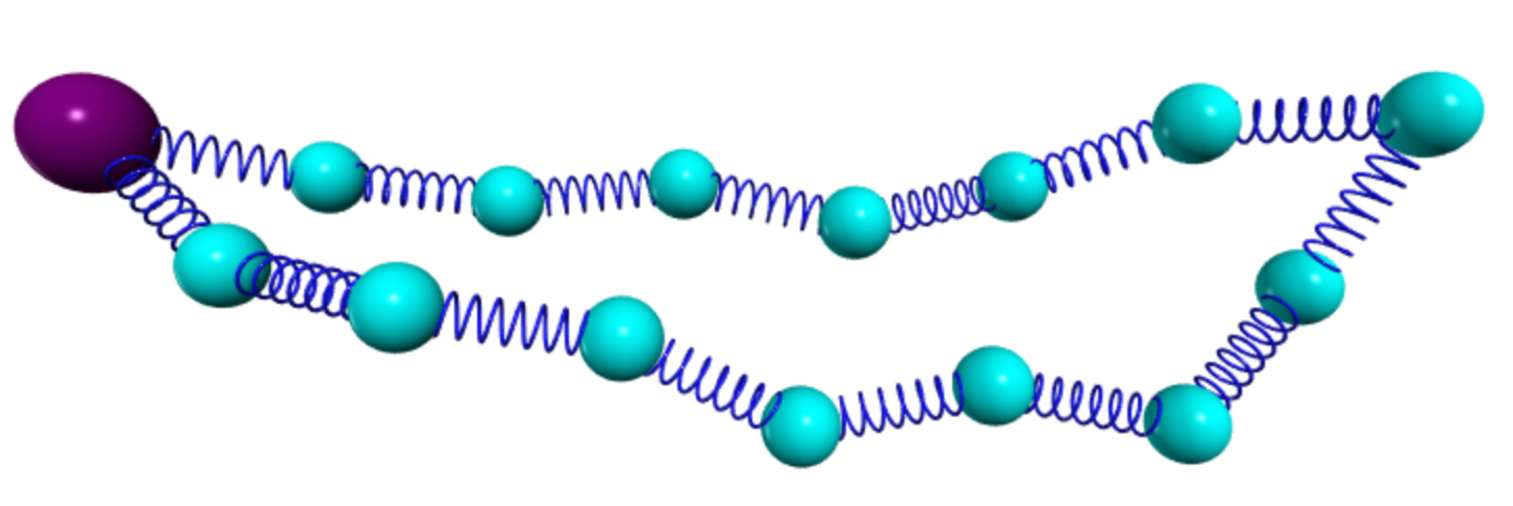
\includegraphics[width=0.8\linewidth]{beadspring}
    \caption{Sketch of the bead-spring loop model. The magenta bead represents the SPB and other cyan beads represent the chromosome segments.}
    \label{fig:beadspring}
\end{figure}

To model the chromosome in fission yeast during nuclear oscillation, we also need a looping structure like the bead-rod model above. The first bead represents the SPB, shown in Fig. \ref{fig:beadspring}. The dynamical equation is similar to the bead-rod model, can be written as following
\begin{equation}
    \label{eq:beadspringEq}
    \xi \frac{d \mathbf{r}_i}{d t} = \mathbf{F}_i^{u} + \mathbf{F}_i^{spring} + \mathbf{F}_i^{e} + \mathbf{F}_i^{b}.
\end{equation}
The notations here are the same as the bead-rod model. In addition, the Brownian force, external force and the potential force are the same as in the bead-rod model. What is different is that the \emph{pseudo} force is not needed and the constraint force is replaced by the spring force $\mathbf{F}_i^{spring}$. Notice that for a bead in the loop, there are two springs connecting to it. Thus
\begin{equation}
    \label{eq:springForce}
    \mathbf{F}_i^{spring} = F_{i+1}^s(Q_{i+1})\mathbf{u}_{i+1} - F_{i}^s(Q_{i})\mathbf{u}_{i},
\end{equation}
here, $F_i^s(Q_i)$ is the tension of the $i^{\rm{th}}$ spring and $Q_i$ is the length of the spring. $\mathbf{u}_i$ is the unit vector for the orientation of the $i^{\rm{th}}$ spring.

There are different types of springs one can use for the model. Here, we will introduce two most commonly used ones and both are used somewhere in the later chapters.

$\bullet$ Hookean spring

Hookean spring is a linear spring, where the tension of spring depends linearly on the length. 
\begin{equation}
    \label{eq:hookeanSpring}
    F^{Hookean} = H (Q-Q_0),
\end{equation}
where $H$ is the Hookean spring constant and $Q_0$ is the natural length of the spring. In practical $Q_0$ is set to $a$, which equals to the length of the bead-rod model. However, sometimes the zero length springs are used. We will point out when needed. 

$\bullet$ Finite Extensible Nonlinear Elastic (FENE) spring

FENE spring is another commonly used spring. The force law of the spring is
\begin{equation}
    \label{eq:feneSpring}
    F^{FENE} = \frac{H Q}{1-(Q/R_0)^2},
\end{equation}
here $R_0$ is the maximal length of the spring. As we can see in Eq. \eqref{eq:feneSpring}, $F^{FENE}\rightarrow\infty$ when $Q\rightarrow R_0$. 


In this section, we specify the dynamics and interaction details of our model for the meiotic chromosomes. The governing equations for the monomers are given. However, we have not talked about the special bead representing the SPB. We will discuss how to pin the SPB in next section.

%********************************** %Second Section  *************************************

\section{Brownian Dynamics simulations}
\label{sec:brownian_dynamics_simulations}
After introducing the model, in this section, we will illustrate how to simulation the model numerically. Since we plan to do most of the theoretical analysis in the later chapters where the simulation results are used for the benchmark, it is convenient that we show the methods of simulation before that. 

Brownian Dynamics (BD) simulation is a kind of Molecule Dynamics (MD) simulation technique. The governing equation of each monomer or particle is integrated to get the trajectories. And physical quantities are measured by ensemble average over trajectories of thousands of monomers. In our situation, the governing equations are Eq. \eqref{eq:beadrodEq} or Eq. \eqref{eq:beadspringEq}. Our interested quantities are something like the average space distance between two beads, the typical size of the polymer and the characteristic time scale of the system dynamics. These are all tractable by BD simulations. 

In the following subsections, we will introduce the algorithms used to do the bead-rod and bead-spring simulation separately. The simulation code is implemented in C++2011. Most the simulation are computed in our clusters with $X86$ architecture.

\subsection{BD simulation of the bead-rod model}
\label{sub:bd_of_bead_rod_model}

Essentially, the goal of the simulation is  to solve the first order ordinary stochastic differential equation Eq. \eqref{eq:beadrodEq} numerically. However, the simple integration algorithm such as the Euler algorithm would not work here. This is because of the implicit constraint force $\mathbf{F}_i^{c}$. Here we employ the predictor-corrector algorithm introduced by Liu \cite{Liu1989}. 

To simplify the illustration of the algorithm, we will ignore all complex potential forces and the external force in Eq. \eqref{eq:beadrodEq}, i.e. $\mathbf{F}_i^{u} = \mathbf{F}_i^{e} = \mathbf{0}$. It is easy to add them back after knowing the algorithm. The dynamical equation after simplification looks 
\begin{equation}
    \label{eq:beadrodSimple}
    \frac{d \mathbf{r}_i}{d t} = \frac{1}{\xi}\left(\mathbf{F}_i^{c} + \mathbf{F}_i^{pseudo} + \mathbf{F}_i^{b}\right).
\end{equation}

The predictor-corrector algorithm is a two-step algorithm and can be divided into the prediction step and correction step. Let us discuss in details.

\subsubsection{Prediction step}
In the prediction step, the estimation of next time step bead position is evaluated without considering the constraints
\begin{equation}
    \label{eq:beadrodPredict}
    \mathbf{r}_i^*(t+\Delta t) = \mathbf{r}_i(t) + \frac{1}{\xi}(\mathbf{F}_i^{pseudo} + \mathbf{F}_i^{b})\Delta t.
\end{equation}
In order to do the calculation, we need to evaluate the Brownian force and the \emph{pseudo} force first. Here we will show how to do that one by one.

$\bullet$ Evaluation of the Brownian force $\mathbf{F}_i^{b}$

The Brownian force is mathematically generated by a Wiener process. Numerically, it is evaluated by a Gaussian distributed \emph{pseudo} random number generated by the computer. Eq. \eqref{eq:beadrodPredict} can be written more practically as 
\begin{equation}
    \begin{aligned}
    \label{eq:beadrodBrownianForce}
    \mathbf{r}_i^*(t+\Delta t) & = \mathbf{r}_i(t) + \frac{1}{\xi}\mathbf{F}_i^{pseudo}\Delta t + \sqrt{\frac{2k_B T}{\xi}}~d\mathbf{W}_i  \\
    & = \mathbf{r}_i(t) + \frac{1}{\xi}\mathbf{F}_i^{pseudo}\Delta t + \sqrt{\frac{2k_B T}{\xi} \Delta t}~\mathbf{N}_i (0, 1),
    \end{aligned}
\end{equation}
where $d\mathbf{W}_i$ is a Wiener process and $\mathbf{N}_i(0,1)$ is a multi-dimensional Gaussian random number of mean $0$ and variance $1$.

$\bullet$ Evaluation of the \emph{pseudo} force $\mathbf{F}_i^{pseudo}$

The expression for \emph{pseudo} force is listed as Eq. \eqref{eq:pseudoForce}. However, the evaluation is not easy and also expensive. To do that, let us first discuss the metric tensor $\mathbf{G}$. 
\begin{equation}
    \label{eq:metricTensor}
    {G}_{\alpha\beta} = \sum_i \frac{\partial g^\alpha}{\partial \mathbf{r}_i} \cdot \frac{\partial g^\beta}{\partial \mathbf{r}_i},
\end{equation}
where $g^\alpha$ is the rigid constraint that 
\begin{equation}
    \label{eq:rigidConstraint}
    g^\alpha(\mathbf{r}_1,\mathbf{r}_2,\cdots,\mathbf{r}_{L}) = 0.
\end{equation}
In the case of a bead-rod loop, Eq. \eqref{eq:rodConstraint} is the constraint. And the $L\times L$ metric tensor looks like
\begin{equation}
    \label{eq:metricMatrix}
    \mathbf{G} = 
    \begin{bmatrix}
        d_1 & c_1 & 0   & \cdots  & c_L \\
        c_1 & d_2 & c_2  &  \cdots & 0 \\
        \vdots & \ddots &\ddots &\ddots &\vdots\\
        0 & \cdots & c_{L-2} & d_{L-1} & c_{L-1} \\
        c_L & \cdots & 0 & c_{L-1} & d_{L}
    \end{bmatrix},
\end{equation}
where diagonal elements $d_i = 2$, and the off-diagonal elements 
\begin{equation}
    c_i = -\mathbf{u}_i\cdot\mathbf{u}_{i-1}
\end{equation}
Again here, the periodic index is applied, i.e. $\mathbf{u}_0 = \mathbf{u}_L$. Now, the \emph{pseudo} force can be calculated as 
\begin{equation}
    \begin{aligned}
    \label{eq:pseudoForceEvaluate}
    \mathbf{F}_i^{pseudo} & = - \frac{1}{2} k_B T \frac{\partial \ln(\det\mathbf{G})}{\partial \mathbf{r}_i} \\
    & = - \frac{1}{2} k_B T \sum_{\alpha,\beta}\frac{1}{\det\mathbf{G}}\frac{\partial\det\mathbf{G}}{\partial{G}_{\alpha\beta}}\frac{\partial{G}_{\alpha\beta}}{\partial\mathbf{r}_i} \\
    & = - \frac{1}{2} k_B T \sum_{\alpha,\beta}{G}_{\beta\alpha}^{-1}\frac{\partial{G}_{\alpha\beta}}{\partial\mathbf{r}_i}.
    \end{aligned}
\end{equation}
In order to calculate the \emph{pseudo} force, we need to inverse the matrix $\mathbf{G}$. This operation is very expensive. Fortunately, the symmetric shape of $\mathbf{G}$ in Eq. \eqref{eq:metricMatrix} makes it possible to find an efficient algorithm to do the computation. We employ the algorithm developed by Pasquali and Morse in \cite{Pasquali2002}. They developed this algorithm for BD simulation of a bead-rod chain. We modified it and successfully applied it to our bead-rod ring model. See Appendix X for details.  

Now the prediction of next time step bead position can be calculated straight forward using Eq. \eqref{eq:beadrodBrownianForce}. The evaluation of other types of forces is quite simple if needed. And we are ready to discuss the correction step.

\subsubsection{Correction step}
The correction step utilizes the result of the prediction, and correct it with the constraint force to obtain the real next time step bead position. 
\begin{equation}
    \label{eq:beadrodCorrect}
    \mathbf{r}_i(t+\Delta t) = \mathbf{r}_i^*(t+\Delta t) + \frac{1}{\xi}\mathbf{F}_i^{c}\Delta t.
\end{equation}
And we known that the rigid rod constraints must be satisfied after the correction. Substitute Eq. \eqref{eq:beadrodCorrect} into Eq. \eqref{eq:rodConstraint} and also notice that 
\begin{equation}
    \label{eq:tensionRod}
    \mathbf{F}_i^{c} = \lambda_{i+1}\mathbf{u}_{i+1} - \lambda_{i}\mathbf{u}_{i}
\end{equation}
where $\lambda_i$ is the magnitude of tension on the $i^{\rm{th}}$ rod. Thus we obtain
\begin{equation}
    \begin{aligned}
    \label{eq:rodTensionEq}
    & 2\Delta t\mathbf{b}_i\cdot\left(\lambda_{i-1}\mathbf{u}_{i-1}-2\lambda_i\mathbf{u}_i+\lambda_{i+1}\mathbf{u}_{i+1}\right) \\
    = &\xi\left(a^2 - \mathbf{b}_i\cdot\mathbf{b}_i\right) -\frac{(\Delta t)^2}{\xi}\left(\lambda_{i-1}\mathbf{u}_{i-1}-2\lambda_i\mathbf{u}_i+\lambda_{i+1}\mathbf{u}_{i+1}\right)^2.
    \end{aligned}
\end{equation}
And $\mathbf{b}_i = \mathbf{r}_i^*(t+\Delta t)- \mathbf{r}_{i-1}^*(t+\Delta t)$. This is a set of nonlinear algebra equations. The second term at the right hand side is the nonlinear term. We can see from here, the nonlinear term is small when the time step $\Delta t$ is small enough. Numerically, it is suitable to use the iteration methods such like the Picard's method to solve this set of equations. High order methods like the Newton's method are also applicable but require the calculation of Jacobian matrix every time step. In practical, a small time step is necessary for the convergence of root searching. We use a time step between $10^{-5}-10^{-3}$ depends on different situations. 

Once we solve the tension $\lambda_i$, plug in to Eq. \eqref{eq:tensionRod} and then Eq. \eqref{eq:beadrodCorrect}, the next time step bead position can be calculated straight forward. 

Finally, We want to discuss a little bit about how to pin the first bead of the bead-rod model. One has several possible ways to do this. The first one is to use a very stiff zero-length spring attached it to the first bead and certain point. This method is very easy to implement. However, the use of the pining spring will introduce a high-frequency factor into the polymer dynamics. This is not good when we analysis of the polymer dynamics. And the spring length is not perfectly zero when the polymer is subjected to a strong force field. So we use another method, i.e. pin the first bead use the zero-length rigid rods. In fact, we will need three this kind of ``ghost'' rods in 3D, the orientation of the rods along three axes respectively. This method requires solving the additional constraint forces. And the calculation is more or less the same as we stated here. With this method, the bead can be pinned perfectly and no disturbing factor will be introduced. 

\subsection{BD simulation of the bead-spring model}
\label{sub:bd_of_bead_spring_model}

The BD simulation of the bead-spring model is much simpler than the bead-rod model. There is neither implicit force nor complex forces need to evaluate during every time step. Of course, one can also use an implicit algorithm which allowed the using of a larger time step. However, we will simply use the explicit algorithms since they work pretty well. 

We will introduce here two simple algorithms to simulate the bead-spring ring polymer, i.e. the Euler method and the stochastic Runge-Kutta method.

\subsubsection{Euler method}

Euler method, also called Euler-Maruyama method, is a 
$1/2$ order integration scheme. In principle, the convergence is only guaranteed when $\Delta t \rightarrow 0$. However, it is still widely used because of its simplicity, especially when the variation of the drift and diffusive term in the stochastic differential equation is not too large. The beads connected by Hookean spring is a good example fits this method. 

Using this method, the next time step bead position in our simple example can be calculated as
\begin{equation}
    \label{eq:beadspringEuler}
    \mathbf{r}_i(t+\Delta t) = \mathbf{r}_i(t) + \frac{1}{\xi}\mathbf{F}_i^{det}\Delta t + \sqrt{\frac{2k_B T}{\xi} \Delta t}~\mathbf{N}_i (0, 1),
\end{equation}
where $\mathbf{F}_i^{det}=\mathbf{F}_i^{u}+\mathbf{F}_i^{spring}+\mathbf{F}_i^{e}$ is the total deterministic force. Also notice that, the $\mathbf{F}_i^{spring}$ is evaluated by Eq. \eqref{eq:springForce} and the spring force law Eq. \eqref{eq:hookeanSpring} or Eq. \eqref{eq:feneSpring}.

\subsubsection{Stochastic Runge-Kutta method}
Stochastic Runge-Kutta method is a higher order integration scheme than the Euler method. It was proposed by Honeycutt in \cite{Honeycutt1992a}. In this method, the next time step bead position can be calculated as
\begin{equation}
    \label{eq:beadspringRK}
    \mathbf{r}_i(t+\Delta t) = \mathbf{r}_i(t) + \frac{1}{\xi}(\mathbf{F}_i^{det}+\tilde{\mathbf{F}}_i^{det})\frac{\Delta t}{2} + \sqrt{\frac{2k_B T}{\xi} \Delta t}~\mathbf{N}_i (0, 1),
\end{equation}
where $\mathbf{F}_i^{det}$ and $\tilde{\mathbf{F}}_i^{det}$ are the total deterministic force evaluated using different bead position.
\begin{equation}
    \begin{aligned}
        \mathbf{F}_i^{det} & = \mathbf{F}_i^{det}\left(\mathbf{r}_0(t),\mathbf{r}_1(t),\cdots,\mathbf{r}_{L-1}(t)\right), \\
        \tilde{\mathbf{F}}_i^{det} & = \tilde{\mathbf{F}}_i^{det}\left(\mathbf{r}_0^*,\mathbf{r}_1^*,\cdots,\mathbf{r}_{L-1}^*\right),
    \end{aligned}
\end{equation}
and $\mathbf{r}_i^*$ is the mid-step bead position
\begin{equation}
    \mathbf{r}_i^*  = \mathbf{r}_i(t) + \frac{1}{\xi}\mathbf{F}_i^{det}\Delta t  + \sqrt{\frac{2k_B T}{\xi} \Delta t}~\mathbf{N}_i (0, 1).
\end{equation}

Last but not least, in the simulations, the dynamical equation is nondimensionalized by rescaling the variable in the following way:
\begin{equation}
    \label{eq:dimensionless}
    \mathbf{r}^{\prime}\to \mathbf{r}/a;~t^{\prime}\to t/(\xi a^2/k_BT);~\mathbf{F}^{\prime}\to\mathbf{F}/(k_BT/a).
\end{equation}
After the rescaling, the length unit is set to the size of the rod. The rescaling is helpful to avoid doing calculations with very small or big numbers, which might introduce larger numerical errors. 


%********************************** % Third Section  *************************************
\section{Monte-Carlo simulation of the bead-rod model}
\label{sec:monte_carlo_simulation_of_the_bead_rod_model}

In the previous section, we present the BD simulation technique of the bead-rod and bead-spring polymer loop. As we can see there, the algorithm used to simulate the bead-rod model is actually quite complex and also time-consuming. Sometimes we do not need to do that if we only want to sample the equilibrium properties of the bead-rod system. In this section, we will introduce a Monte-Carlo algorithm that is much faster and efficient to obtain the equilibrium statistics of the bead-rod loop model. 

Monte-Carlo technique has used to simulate the polymer system for a long time \cite{Binder1995}. However, there are some special factors one need to take into account for our pinned polymer loop model. Basically, one has to preserve the loop structure and keep the rod length fixed when trying to do a Monte-Carlo flip. According to this, we propose the following main steps of our Monte-Carlo algorithm. 

$\bullet$ Step I: prepare an initial configuration and compute the energy of this configuration. The way of calculating system energy depends on the setting of the model, whether the excluded volume effect or other interactions are taken into account or not. For example, the energy of a pinned bead-rod loop in a constant external force field can be written as
\begin{equation}
    \label{eq:mcEnergy}
    E = U - \sum_{i=1}^L\mathbf{F}^{e} \cdot \mathbf{r}_i
\end{equation}
where $U$ is other kind of interaction energy. In the simplest case, we will assume $U$ is independent of the configurations. To compare with the later evaluation, we denote the energy calculated here $E_{old}$.

$\bullet$ Step II: randomly choice two beads in the polymer loop, use the connecting line between the two beads as a rotation axis.
\begin{figure}[htpb]
    \centering
    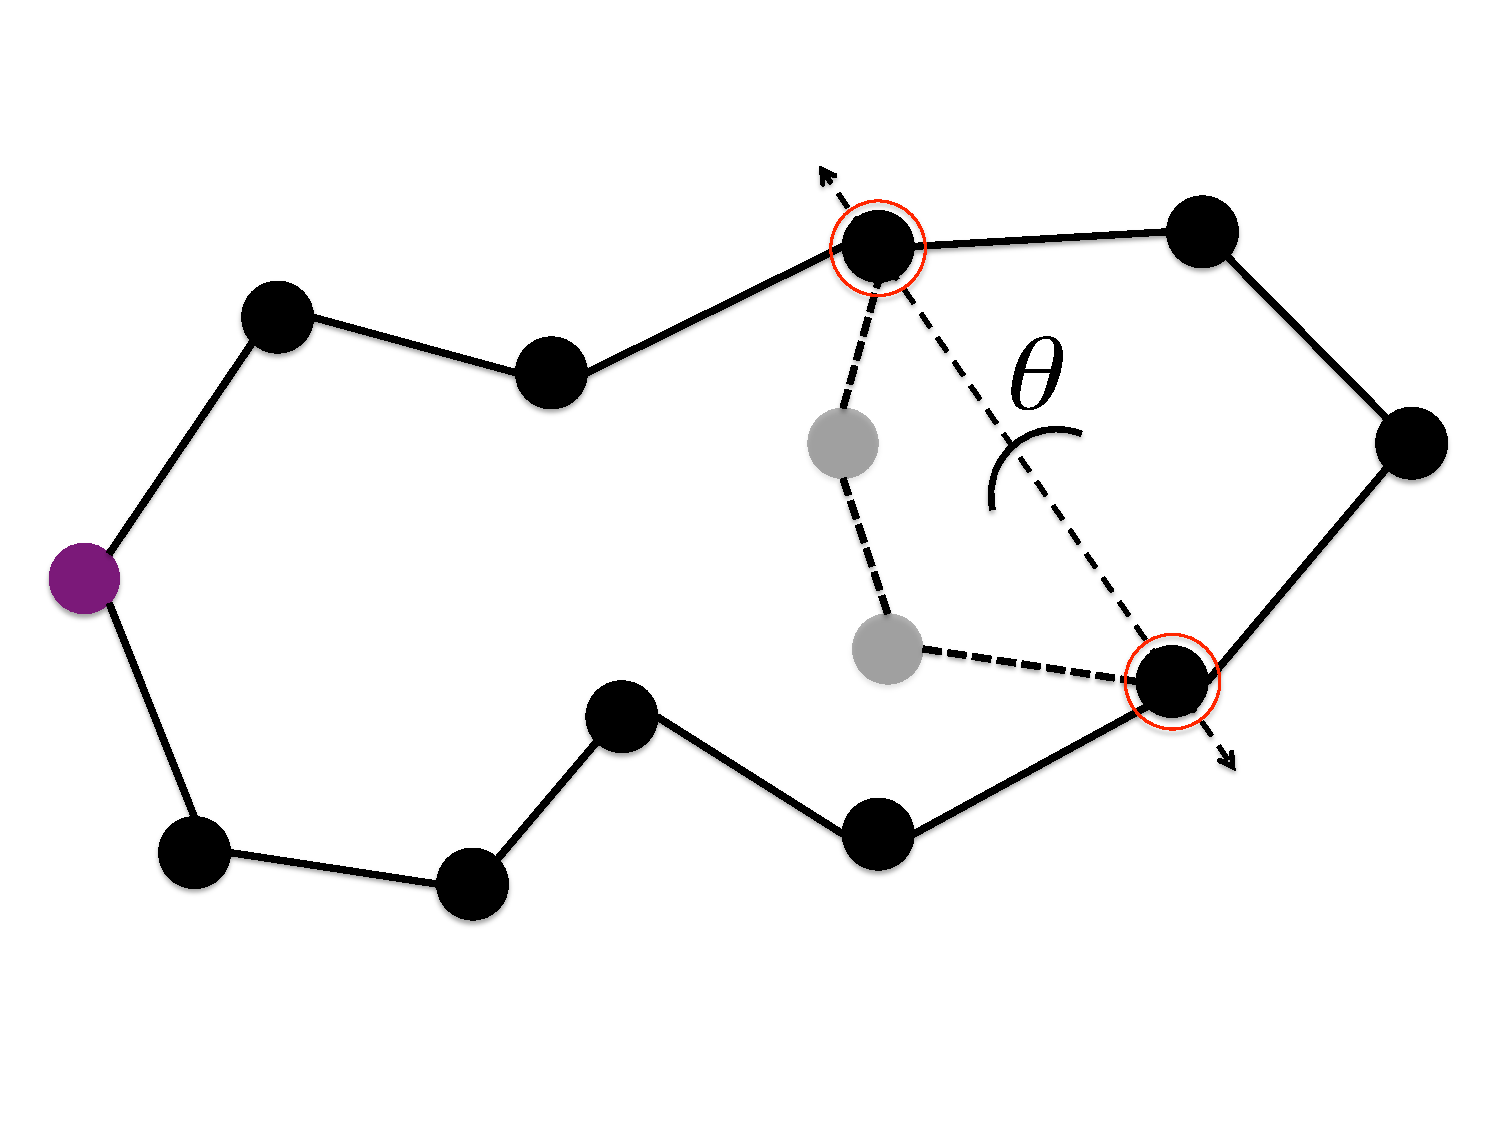
\includegraphics[width=0.8\linewidth]{rotation}
    \caption{Illustration of the Monte-Carlo configuration flip. }
    \label{fig:rotation}
\end{figure}

$\bullet$ Step III: choose the unpinned side of the polymer, and rotate this part of the polymer by a random angle $\theta\in[-\phi, \phi]$. $\phi$ is a parameter between $[0,\pi]$ and can be tuned to improve the efficiency of the algorithm. See in Fig. \ref{fig:rotation}. If the pinned bead is selected, then randomly choose a side of the polymer to do the rotation. 

$\bullet$ Step IV: calculated the energy of the configuration after rotation in the same way of $E_{old}$. Let us denote the new energy as $E_{new}$.

$\bullet$ Step V: the new configuration is accepted with probability  
\begin{equation}
    \label{eq:mcProbability}
    p = \min\left\{1, \exp\left(-\frac{\Delta E}{k_BT}\right)\right\},
\end{equation}
where $\Delta E = E_{new} - E_{old}$. If not accepted, then the polymer returns to the old configuration, and try again with new random number. An efficient sampling algorithm can be tuned by parameter $\phi$ so that the accept probability is around $0.5$.

$\bullet$ Step VI: go back to step I and loop again and again to get enough independent samples. Physical quantities such like the statistical distance between two beads can be calculated by averaging over these samples.

The Monte-Carlo method introduced in this section is efficient and fast, we will use it to calculate most of the equilibrium quantities in next chapter. On the other hand, the Monte-Carlo results also work as a benchmark of the BD simulation and vice-versa. 


%********************************** % Fourth Section  *************************************

\section{Summary}
\label{sec:summary_chap2}

In this chapter, we elaborated the details of our pulled polymer model for the chromosomes in meiotic fission yeast. We have shown that the pulled polymer loop is equivalent to the pinned polymer loop in external force field after a coordinate transform. The concrete bead-rod and bead-spring polymer loop models are discussed. And the BD simulation technique is discussed in details. A Monte-Carlo algorithm is introduced to calculate the equilibrium statistics of the bead-rod system and overcomes the disadvantages of heavy computation for the BD simulation.

The content of this chapter will be very useful in our later chapters. And we try to keep it concise, many related interesting models or methods are not mentioned here. Only those that will use in this thesis are discussed. Interested readers can refer to the cited references.

In next chapter, we will start to discuss the theory of equilibrium statistics of our polymer model and use the theory to explain the chromosome alignment in fission yeast. 
